\documentclass{beamer}
\usepackage{siunitx}

\usepackage[utf8]{inputenc}
\usetheme{Warsaw}
\title{MATRIX PROJECT}
\author{JAYANT RANGI(MA17BTECH11006) \newline RITESH YADAV(MA17BTECH11009) }


\begin{document}

\maketitle
\begin{frame}{QUESTION:}
The sides of a rhombus ABCD are parallel to the lines
\newline
\begin{itemize}
\item (1,-$1$) \textbf{X} + 2 = 0
\item (7,-$1$) \textbf{X} + 3 = 0
\end{itemize}
If the diagonals of the rhombus intersect at
\newline

\textbf{P} = 
\(
\begin{bmatrix}
1\\
2\\
\end{bmatrix}
\)
and the vertex A (different) from the origin is
on the y-axis, then find the ordinate of A.



    
\end{frame}
\begin{frame}{SOLUTION APPROACH (USING VECTORS) :}
For line: (1,-$1$) \textbf{X} + 2 = 0 \newline
Let 
\textbf{N}_1 
= 
\(
\begin{bmatrix}
\frac{1}{\sqrt{2}}\\
\frac{-1}{\sqrt{2}} \\
\end{bmatrix}
\)
be the \textbf{normal unit vector}.
\newline
\newline
\newline
For line: (7,-$1$) \textbf{X} + 3 = 0 \newline
Let 
\textbf{N}_2 
= 
\(
\begin{bmatrix}
\frac{7}{5\sqrt{2}}\\
\frac{-1}{5\sqrt{2}} \\
\end{bmatrix}
\)
be the \textbf{normal unit vector}.
    
\end{frame}
\begin{frame}{Vector Addition}
\centering 
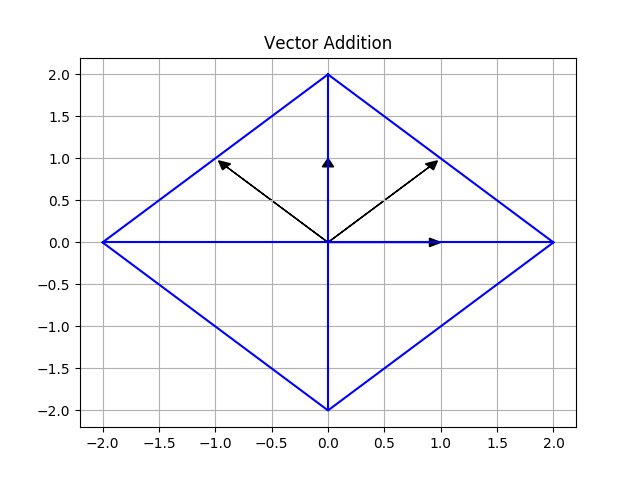
\includegraphics[scale=0.6]{graph1.png}
\end{frame}

\begin{frame}{}

Let $D_1$  and $ D_2 $ be the vectors along diagonals of the Rhombus ABCD and A will be on one of the diagonals.
\newline
By parallelogram law of vector addition:
\newline
\newline
\textbf{D}_1 = \textbf{N}_1 + \textbf{N}_2 =
\(
\begin{bmatrix}
\frac{12}{5\sqrt{2}}\\
\frac{-6}{5\sqrt{2}} \\
\end{bmatrix}
\)
\newline
\newline

\textbf{D}_2 = \textbf{N}_2 - \textbf{N}_1 =
\(
\begin{bmatrix}
\frac{2}{5\sqrt{2}}\\
\frac{4}{5\sqrt{2}} \\
\end{bmatrix}
\)

\end{frame}

\begin{frame}{Equation of Diagonals:}
Diagonal along $\textbf{D}_1$ passing through point \textbf{P}:
\newline
\newline
$\textbf{D}_2$^T\textbf{X} =  $ \textbf{D}_2$^T$\textbf{P} $    ( Because $ \textbf{D}_2 $ is normal to $\textbf{D}_1$ )
\newline
\newline
\(
\begin{bmatrix}
\frac{2}{5\sqrt{2}}&\frac{4}{5\sqrt{2}}\\
\end{bmatrix}
\)\textbf{X} = $\frac{10}{5\sqrt{2}}$
\newline
\newline
Diagonal along $\textbf{D}_2$ passing through point \textbf{P}:
\newline
\newline
$\textbf{D}_1$^T\textbf{X} =  $ \textbf{D}_1$^T$\textbf{P} $    ( Because $ \textbf{D}_1 $ is normal to $\textbf{D}_2$ )
\newline
\newline
\(
\begin{bmatrix}
\frac{12}{5\sqrt{2}}&\frac{-6}{5\sqrt{2}}\\
\end{bmatrix}
\)\textbf{X} = 0
\end{frame}
\begin{frame}{Diagonals of Rhombus}

\centering
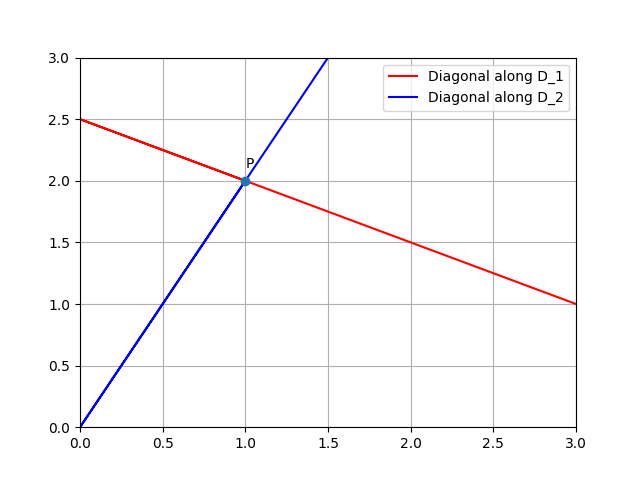
\includegraphics[scale=0.6]{graph2.png}
    
\end{frame}
\begin{frame}{Result:}
As the Diagonal along $\textbf{D}_2$ passes through origin so we will neglect it as according to question point A can not be origin.
\newline
\newline
Hence , A is the point where Diagonal along $\textbf{D}_1$ intersects y-axis. So:
\newline
\newline
\(
\begin{bmatrix}
\frac{2}{5\sqrt{2}}&\frac{4}{5\sqrt{2}}\\
\end{bmatrix}
\)\textbf{X} = $\frac{10}{5\sqrt{2}} $
, where \textbf{X} = \(
\begin{bmatrix}
0\\
y \\
\end{bmatrix}
\)
\newline
\newline
Therefore, y = $\frac{5}{2} $ (i.e ordinate of A)
\newline
\newline
Point \textbf{A} is (0,$\frac{5}{2} $). 

    
\end{frame}
\begin{frame}{Rhombus ABCD}
\centering
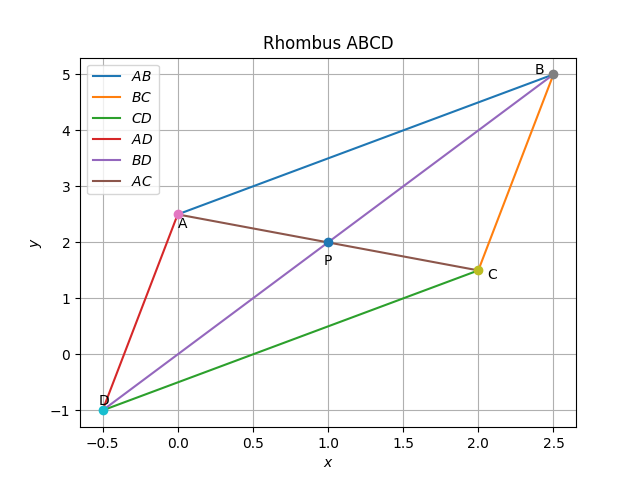
\includegraphics[scale=0.6]{graph3.png}
    
\end{frame}

\section{Introduction}

\end{document}
